\begin{tikzpicture}[ele/.style={fill=black,circle,minimum width=.8pt,inner sep=1pt},every fit/.style={ellipse,draw,inner sep=15},scale=0.6, every node/.style={scale=0.6}]
    \draw[white] (0,0);
    \node[ele,label=left:$1$] (a1) at (0,4) {};    
    \node[ele,label=left:$2$] (a2) at (0,3) {};    
    \node[ele,label=left:$3$] (a3) at (0,2) {};
    \node[ele,label=left:$4$] (a4) at (0,1) {};
    
    \node[ele,,label=right:$1$] (b1) at (4,4) {};
    \node[ele,,label=right:$2$] (b2) at (4,3) {};
    \node[ele,,label=right:$3$] (b3) at (4,2) {};
    \node[ele,,label=right:$4$] (b4) at (4,1) {};
    
    \node[draw,fit= (a1) (a2) (a3) (a4),minimum width=2cm] {} ;
    \node[draw,fit= (b1) (b2) (b3) (b4),minimum width=2cm] {} ;  
    \draw[->,thick,shorten <=2pt,shorten >=2pt] (a1) -- (b1);
    \draw[->,thick,shorten <=2pt,shorten >=2] (a2) -- (b4);
    \draw[->,thick,shorten <=2pt,shorten >=2] (a3) -- (b2);
    \draw[->,thick,shorten <=2pt,shorten >=2] (a4) -- (b3);
\end{tikzpicture}
\hspace{2cm}
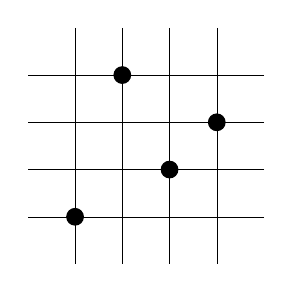
\begin{tikzpicture}[,scale=0.6, every node/.style={scale=0.6}]
        \foreach \x in {1,...,4} {
                \draw[ultra thin] (\x,5)--(\x,0);
                \draw[ultra thin] (5,\x)--(0,\x);
        }
        \draw[fill=black] (1,1) circle (5pt);
        \draw[fill=black] (2,4) circle (5pt);
        \draw[fill=black] (3,2) circle (5pt);
        \draw[fill=black] (4,3) circle (5pt);
\end{tikzpicture}